
\documentclass[11pt, a4paper, twoside]{article}   	% use "amsart" instead of "article" for AMSLaTeX format

\usepackage{geometry}                		% See geometry.pdf to learn the layout options. There are lots.
\usepackage{pdfpages}
\usepackage{listings}				% For Source Code displaying
\usepackage[german]{babel}			% this end the next are needed for german umlaute
\usepackage[utf8]{inputenc}
\usepackage{color}
\usepackage{graphicx}
\usepackage{titlesec}
\usepackage{fancyhdr}
\usepackage{lastpage}
\usepackage{hyperref}
% http://www.artofproblemsolving.com/wiki/index.php/LaTeX:Symbols#Operators
% =============================================
% Layout & Colors
% =============================================
\geometry{
   a4paper,
   total={210mm,297mm},
   left=20mm,
   right=20mm,
   top=20mm,
   bottom=30mm
 }	

\definecolor{myred}{rgb}{0.8,0,0}
\definecolor{mygreen}{rgb}{0,0.6,0}
\definecolor{mygray}{rgb}{0.5,0.5,0.5}
\definecolor{mymauve}{rgb}{0.58,0,0.82}

\setcounter{secnumdepth}{4}


% the default java directory structure and the main packages
\newcommand{\srcDir}{../src/main/java}
\newcommand{\srcTestDir}{../src/test/java}
\newcommand{\mainPackage}{\srcDir/at/fhooe/swe4/lab3}
\newcommand{\mainTestPackage}{\srcTestDir/at/fhooe/swe4/lab3/test}
\newcommand{\imagesDir}{images}
% the default subsection headers
\newcommand{\ideaSection}{Lösungsidee}
\newcommand{\sourceSection}{Source-Code}
\newcommand{\testSection}{Tests}
% text fragemnt fpr test section
\newcommand{\testCommonText}{Diese Test wurden mit Hilfe von JUnit in der Entwicklungsumgebung Eclipse implementiert, daher können diese Tests einfach in einer Eclipse Umgebung reproduziert werden.\\ 
Die angezeigten Berechnungszeiten sind abhängig von der verwendeten Hardware.}
% sort common test text
\newcommand{\testSortCommonText}{
Die Zeitmessungen wurden in einem eigenen Punkt zusammengefasst, da hier beide Sortieralgorithmen Algorithmen gegeneinander verglichen werden.
}

% =============================================
% Code Settings
% =============================================
\lstdefinestyle{sourceFileStyle}{ %
  basicstyle=\footnotesize,        % the size of the fonts that are used for the code
  breakatwhitespace=false,         % sets if automatic breaks should only happen at whitespace
  breaklines=true,                 % sets automatic line breaking
  captionpos=t,                    % sets the caption-position to top
  commentstyle=\color{mygreen},    % comment style
  frame=single,                    % adds a frame around the code
  keepspaces=true,                 % keeps spaces in text, useful for keeping indentation of code (possibly needs columns=flexible)
  keywordstyle=\color{blue},       % keyword style
  language=JAVA, 
  numbers=left,                    % where to put the line-numbers; possible values are (none, left, right)
  numbersep=5pt,                   % how far the line-numbers are from the code
  numberstyle=\tiny\color{mygray}, % the style that is used for the line-numbers
  rulecolor=\color{white},         % if not set, the frame-color may be changed on line-breaks within not-black text (e.g. comments (green here))
  showspaces=false,                % show spaces everywhere adding particular underscores; it overrides 'showstringspaces'
  showstringspaces=false,          % underline spaces within strings only
  showtabs=false,                  % show tabs within strings adding particular underscores
  stepnumber=1,                    % the step between two line-numbers. If it's 1, each line will be numbered
  stringstyle=\color{mymauve},     % string literal style
  tabsize=2,                       % sets default tabsize to 2 spaces
  title=\lstname                   % show the filename of files included with \lstinputlisting; also try caption instead of title
}
\lstdefinestyle{inlineSource}{ 
  basicstyle=\footnotesize,
  breakatwhitespace=false,
  breaklines=true,
  keepspaces=true,   
  commentstyle=\color{mygreen},
  keywordstyle=\color{blue},
  language=JAVA
}
\newcommand{\inlinecode}{\lstinline[style=inlineSource]}
% =============================================
% Page Style, Footers & Headers, Title
% =============================================
\title{Übung 3}
\author{Thomas Herzog}

\lhead{Übung 3}
\chead{}
\rhead{
\includegraphics[scale=0.10]{FHO_Logo_Students.jpg}}

\lfoot{S1310307011}
\cfoot{}
\rfoot{ \thepage / \pageref{LastPage} }
\renewcommand{\footrulewidth}{0.4pt}
% =============================================
% D O C U M E N T     C O N T E N T
% =============================================
\pagestyle{fancy}
\begin{document}
\setlength{\headheight}{15mm}
% =============================================
% Solution Idea
% =============================================
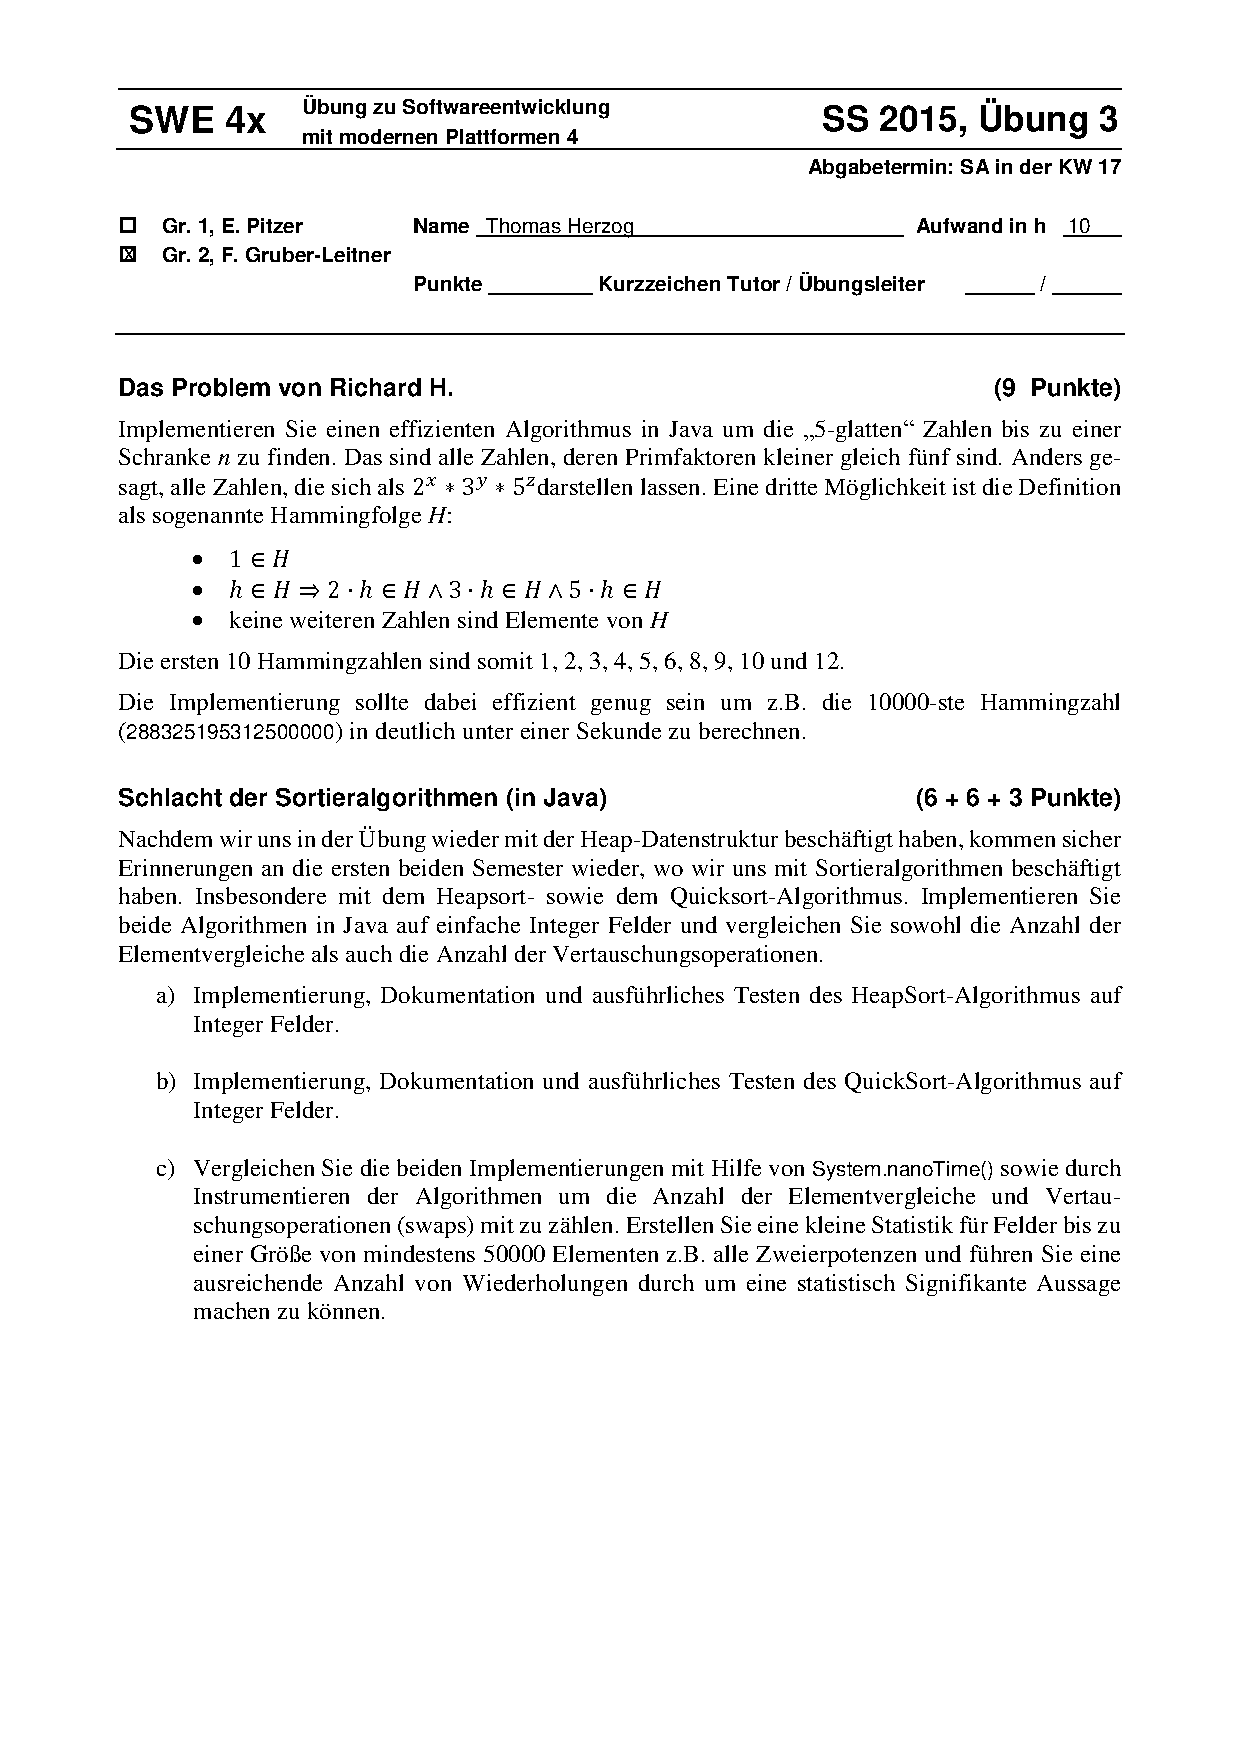
\includepdf[pages={1}]{Java_1.pdf}
{\color{myred}
	\section
		{Hammingfolge}
}
% =============================================
% 1. Hamming numbers
% =============================================
% Idea
% =============================================
\subsection{\ideaSection}
Folgend ist die Lösungsidee für die Aufgabenstellung Berechnung einer Hammingfolge angeführt.\\
Da es sich hierbei lediglich um einen einzigen Algorithmus handelt soll dieser als Klassenmethode implementiert werden. Das diese Klasse lediglich diese Klasenmethode enthalten soll, soll in dieser Klasse ein Privater Konstruktor \inlinecode|private Hamming () {}| implementiert werden um zu verhindern, dass diese Klasse instanziert werden kann.\\\\
Da eine Hammingfolge wie folgt definiert ist:\\
$1 \in H$ \\
$x \in H \Rightarrow 2 \ast x \in H \wedge 3 \ast x \in H \wedge 5 \ast x \in H$\\
wissen wir dass folgende Elemente aufgrund dessen das $1 \in H$ gilt in der Folge vorhanden sind. \\
$1 \in H \wedge 2 \in H \wedge 3 \in H \wedge 5 \in H$\\
daher können wir einen Algorithmus definieren der sich wie folgt verhalten soll:
\begin{enumerate}
	\item Instanziere eine \inlinecode{NavigableSet<E>} und initialisiere dieses Set mit dem Element 1
	\item Instanziere eine \inlinecode{List<E>} welches die resultierenden Werte beinhaltet wird
	\item Polle und entferne das erste Element aus dem Set
	\item Füge dieses Element der resultierenden Liste hinzu.		
	\item Berechne die nachfolgenden Hammingzahlen $(2 \ast polledValue \wedge 3 \ast polledValue \wedge 5 \ast polledValue)$ für dieses Element
	\item Füge die Berechneten Elemente der \inlinecode{Navigable<E>} Instanz hinzu
	\item Wiederhole Schritt 3 solange folgendes gilt:  \inlinecode{resultList.size(i) < n}
\end{enumerate}
Es soll gegen \inlinecode{NavigableSet<E>} Interface und nicht gegen \inlinecode{SortedSet<E>} gearbeitet werden, da dieses Interface eine Methode namens \inlinecode{instance.pollFirst()} zur Verfügung stellt, die das erste Element des \inlinecode{NavigableSet<E>} liefert und es gleichzeitig aus dem \inlinecode{NavigableSet<E>} entfernt. Für das zu verwendende Interface \inlinecode{NavigableSet<E>} soll eine \inlinecode{TreeSet<E>} Instanz verwendet werden.  Dadurch sollte der Container in seiner Größe beschränkt werden, was den Sortierungsaufwand des Containers minimal halten sollte.\\
Da \inlinecode{TreeSet<E>} aber auch \inlinecode{SortedSet<E>} implementiert sind die enthaltenen Werte implizit immer sortiert und dadurch auch die Werte in der resultierenden Liste, da die hinzugefügten Elemente immer sortiert eingefügt werden. Es ist nicht notwendig einen eigenen \inlinecode{Comparator<E>} zu implementieren da die natürliche Ordnung der \inlinecode{BigInteger} Instanzen ausreicht (Implementiert das Interface \inlinecode{Comparable<E>}). 
\newpage
% =============================================
% Source
% =============================================
\subsection{\sourceSection}
Folgend ist der implementierte Source und Test-Source angeführt.
\lstinputlisting[style=sourceFileStyle]{\mainPackage/hamming/Hamming.java}
\lstinputlisting[style=sourceFileStyle]{\mainTestPackage/hamming/HammingTest.java}
% =============================================
% Tests
% =============================================
\newpage
\subsection{\testSection}
Folgend sind die Tests der Aufgabenstellung Berechnen einer Hammingfolge angeführt.\\
\testCommonText
\begin{figure}[h]
  \centering
  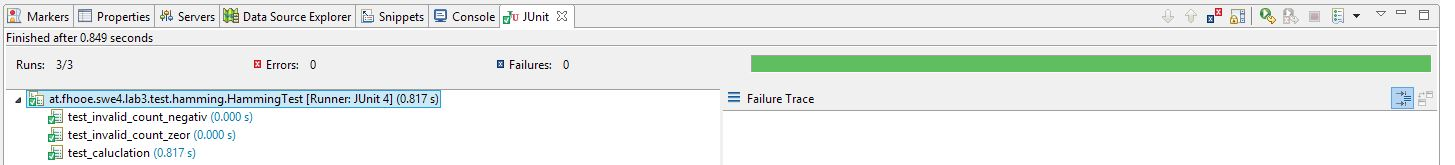
\includegraphics[width=\textwidth]{\imagesDir/tests_hamming_junit.JPG}
  \caption[JUnit Reulstat]
   {Diese Abbildung zeigt das Resultat der JUnit Tests im Eclipse}
\end{figure}
\begin{figure}[h]
  \centering
  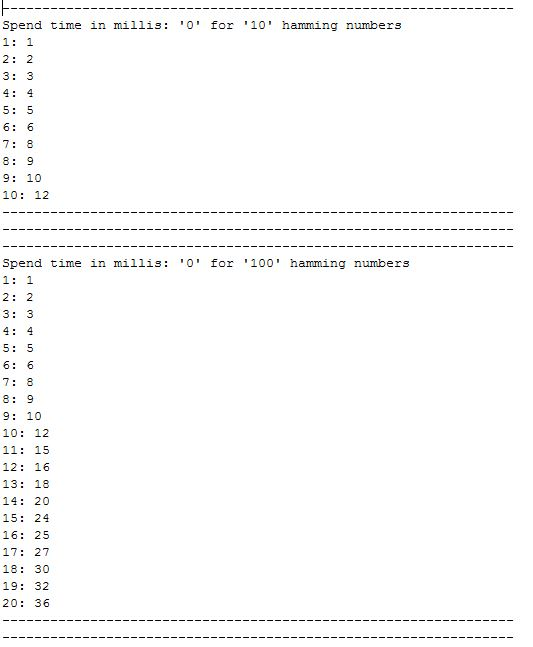
\includegraphics[scale=0.8]{\imagesDir/tests_hamming_console_1.JPG}
  \caption[Konsolenausgabe der Berechnungszeiten]
   {Diese Abbildung zeigt die Berechnungszeiten für 10, 100 Hammingzahlen}
\end{figure}
\newpage
\begin{figure}[h]
  \centering
  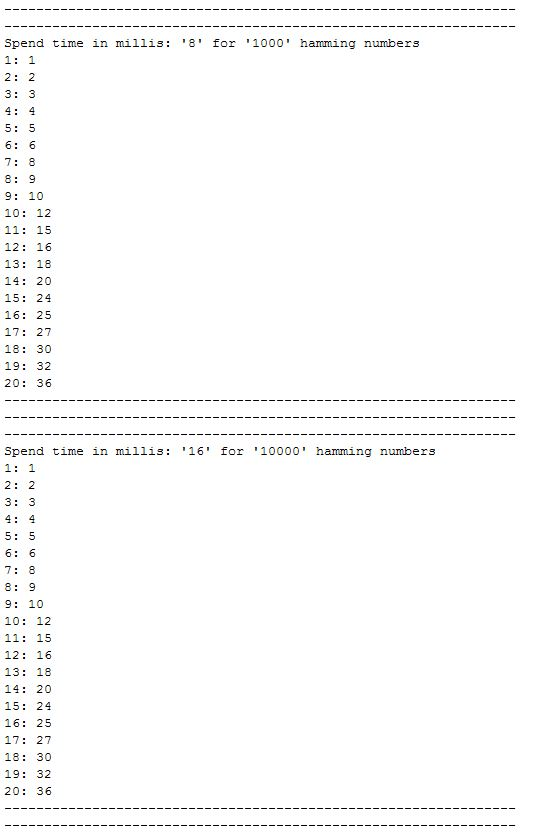
\includegraphics[scale=0.8]{\imagesDir/tests_hamming_console_2.JPG}
  \caption[Konsolenausgabe der Berechnungszeiten]
   {Diese Abbildung zeigt die Berechnungszeiten für 1000, 10.000 Hammingzahlen}
\end{figure}
\newpage
\begin{figure}[h]
  \centering
 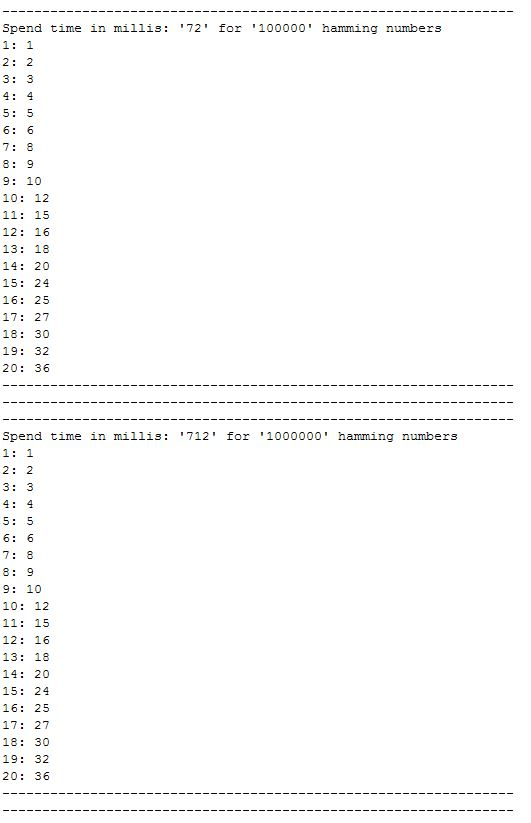
\includegraphics[scale=0.8]{\imagesDir/tests_hamming_console_3.JPG}
  \caption[Konsolenausgabe der Berechnungszeiten]
   {Diese Abbildung zeigt die Berechnungszeiten für 100.000, 1.000.000 Hammingzahlen}
\end{figure}
% =============================================
% 2. Sorting algorithms
% =============================================
% Idea (common)
% =============================================
\newpage
{\color{myred}
	\section
		{Sortieralgorithmen}
}
\subsection{\ideaSection \hspace{2mm}(Allgemein)}
Folgend sind die Lösungsideen der Sortierlagorithmen HeapSorter und QuickSorter angeführt.\\
Da beide Algorithmen denselben output liefern sollen, soll hier ein Interface spezifiziert werden welches die Funktionalität bzw. die zu implementierenden Methoden Signaturen vorgibt. Die Aufgabenstellung verlangt zwar nur das Sortieren auf Integer Felder, jedoch sollen die Algorithmen so implementiert werden, dass sie auf Typen, die das Interface \inlinecode{Compareable<E>} implementieren, angewendet werden können.\\
Daher muss das Interface folgende Signatur vorweisen.\inlinecode|public Sorter<E extends Comparable<E>> {...}|
\newpage
% =============================================
% Source (common)
% =============================================
\newpage
\subsubsection{Source Code\hspace{2mm}(Allgemein)}
Folgend ist der Source des Interface Sorter angeführt
\lstinputlisting[style=sourceFileStyle]{\mainPackage/sort/api/Sorter.java}
\newpage
% =============================================
% 2.1 Statistics
% =============================================
% Idea (stastistics)
% =============================================
\subsection{\ideaSection \hspace{2mm}(Statistics)}
Aufgrund dessen dass die Sortieralgorithmen mit Code Statistics versehen werden sollen, sollen Klassen implementiert werden, die es erlauben die verlangten Statistiken zu ermitteln und auch einen Report dieser zu generieren.\\
Hierbei soll diese Code Statistik Ressourcen wie folgt aufgeteilt werden:
\begin{enumerate}
	\item \textbf{StatisticsProvider:} Das Interface welches die Spezifikation für den Code Statistik Provider enthalten soll.\\
	Die Implementierung soll es ermöglichen mehrere Statistik Kontexte zu verwalten.
	\item \textbf{StatisticContext:} Die Klasse, welche einen Statistik Kontext darstellen soll.\\
	Dieser Kontext soll es ermöglichen mehrere CodeStatistic Instanzen pro Kontext zu verwalten.
	\item \textbf{CodeStatistic:} Die Klasse, die die Code Statistik Informationen (swap, compare counts) halten soll
	\item \textbf{DefaultStatisticProviderImpl:} Die default Implementierung des Interface StatisticProvider, welches die Funktionalitäten implementiert soll.
\end{enumerate}
Alle Klassen sollen die \inlinecode{instance.toString()}  Methode überschreiben und jeweils ihre beinhaltenden Informationen als \inlinecode{String} zurückliefern, wobei ein Parent bzw. die Instanz, die Instanzen verwaltet, an deren \inlinecode{child.toString()} zu delegieren hat.
\newpage
% =============================================
% Idea (statistics)
% =============================================
\newpage
\subsubsection{Source Code}
Folgend ist der Source der Statistik Interfaces und Implementierungen angeführt.
\lstinputlisting[style=sourceFileStyle]{\mainPackage/stat/api/StatisticsProvider.java}
\lstinputlisting[style=sourceFileStyle]{\mainPackage/stat/StatisticContext.java}
\lstinputlisting[style=sourceFileStyle]{\mainPackage/stat/CodeStatistics.java}
\lstinputlisting[style=sourceFileStyle]{\mainPackage/stat/DefaultStatisticsProviderImpl.java}

% =============================================
% 2.2 HeapSorter
% =============================================
% Idea (heapsorter)
% =============================================
\newpage
\subsection{HeapSorter}
Folgend ist die Lösungsidee für die HeapSorter Implementierung angeführt.\\
Da hierbei eine Heap Implementierung von Nöten ist und diese aber auch anderweitig verwendet werden könnte, soll ein Heap Implementiert werden, der unabhängig von einem HeapSorter verwendet werden kann. Da wir auch hier generisch bleiben wollen und es auch möglich sein soll eine Heap Implementierung mit einem anderen Container zu implementieren (Bsp.: \inlinecode{ArrayList<E>}, \inlinecode{T[]}, usw.) soll ein Interface spezifiziert werden, welches die Funktionalitäten eines Heap spezifiziert.\\ Es soll folgende Signatur haben
\inlinecode|public Heap<E extends Comparable<E>> {...}|\\
Des Weiteren soll eine Enumeration spezifiziert werden, die es erlaubt zu definieren, ob der Heap ein upheap oder downheap sein soll, also ob der root das höchste oder kleinste Element darstellt.\\
Ansonsten soll der Heap wie bekannt implementiert werden.
% =============================================
% Source(heapsorter)
% =============================================
\newpage
\subsubsection{Source Code}
Folgend ist der Source der Interfaces und Implementierungen für Heap und HeapSorter angeführt.
\lstinputlisting[style=sourceFileStyle]{\mainPackage/sort/api/Heap.java}
\lstinputlisting[style=sourceFileStyle]{\mainPackage/sort/heap/impl/HeapArrayListImpl.java}
\lstinputlisting[style=sourceFileStyle]{\mainPackage/sort/heap/impl/HeapSorter.java}
% =============================================
% Tests (heapsorter)
% =============================================
\newpage
\subsubsection{\testSection}
Folgend sind die Tests für die HeapSorter Implementierung angeführt.\\
\testCommonText\\
\testSortCommonText
\begin{figure}[h]
  \centering
  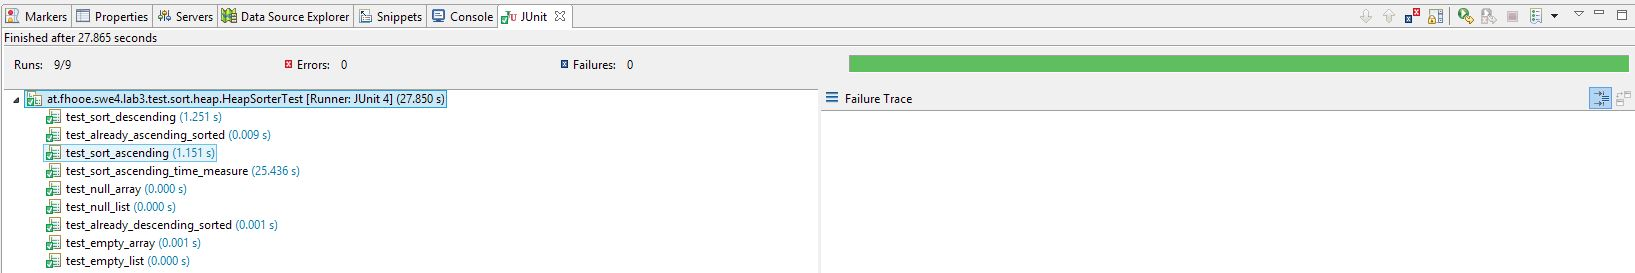
\includegraphics[width=\textwidth]{\imagesDir/tests_heap_junit.JPG}
  \caption
   {Diese Abbildung zeigt das Resultat der JUnit Tests im Eclipse}
\end{figure}
\newpage
\begin{figure}[h]
  \centering
  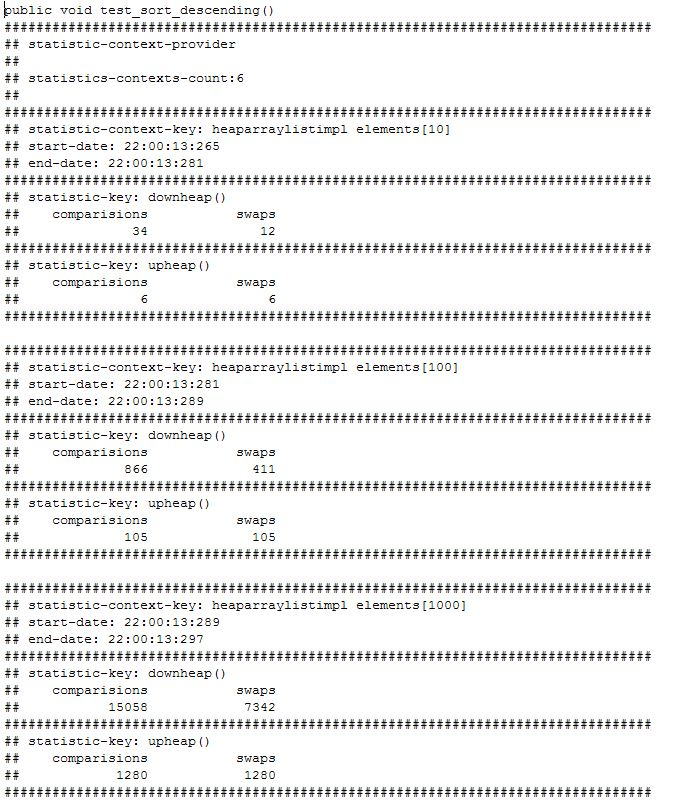
\includegraphics[scale=0.8]{\imagesDir/tests_heap_console_1.JPG}
  \caption
   {Diese Abbildung zeigt die Statistiken für das absteigende Sortieren von 10, 100, 1.000 Elementen}
\end{figure}
\newpage
\begin{figure}[h]
  \centering
  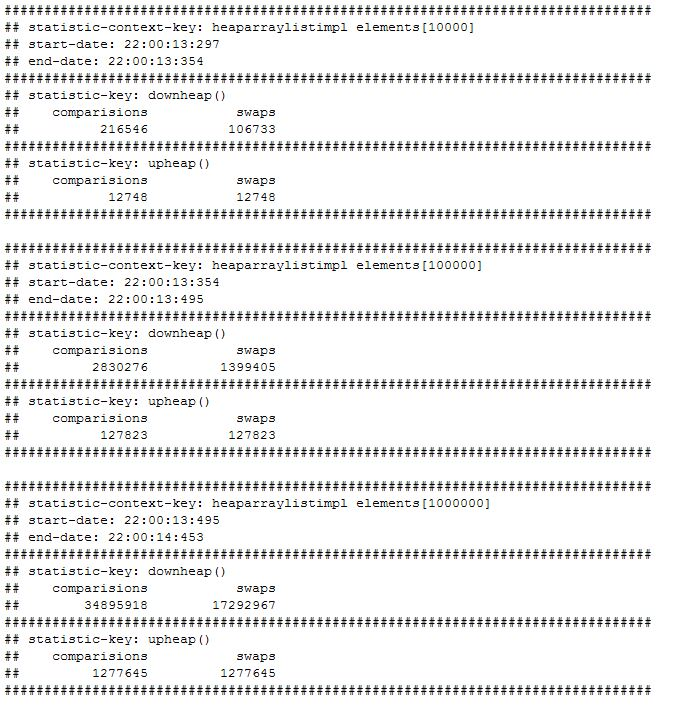
\includegraphics[scale=0.8]{\imagesDir/tests_heap_console_2.JPG}
  \caption
   {Diese Abbildung zeigt die Statistiken für das absteigende Sortieren von 10.000, 100.000, 1.000.000 Elementen}
\end{figure}
\newpage
\begin{figure}[h]
  \centering
  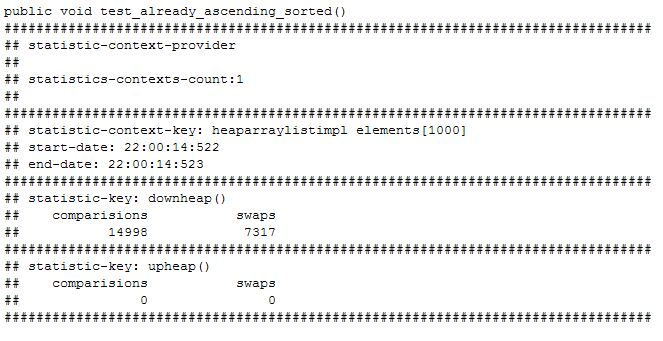
\includegraphics[scale=0.8]{\imagesDir/tests_heap_console_3.JPG}
  \caption
   {Diese Abbildung zeigt die Statistiken für das aufsteigende Sortieren von 1.000 Elementen, die bereits aufsteigend sortiert sind}
\end{figure}
\newpage
\begin{figure}[h]
  \centering
  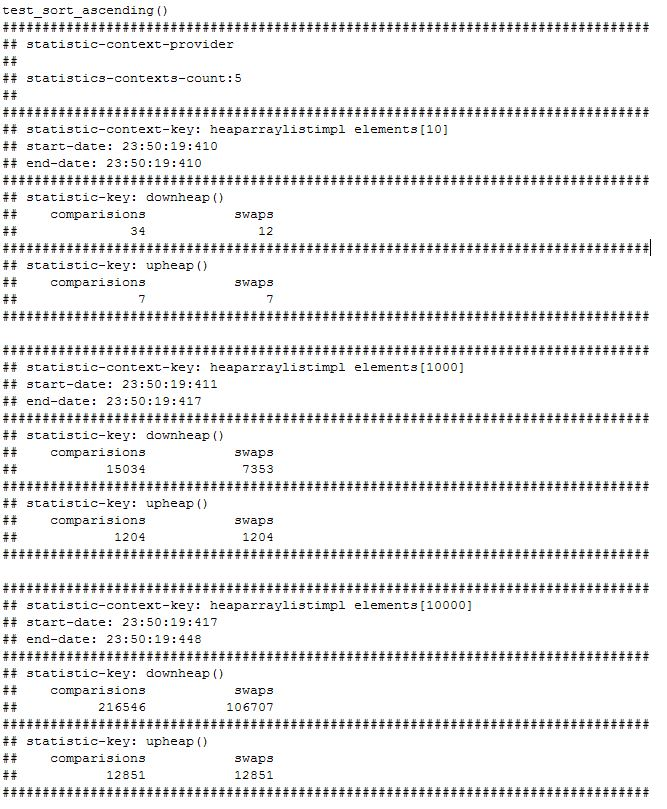
\includegraphics[scale=0.8]{\imagesDir/tests_heap_console_4.JPG}
  \caption
   {Diese Abbildung zeigt die Statistiken für das aufsteigende Sortieren von 10, 100, 1.000 Elementen}
\end{figure}
\newpage
\begin{figure}[h]
  \centering
  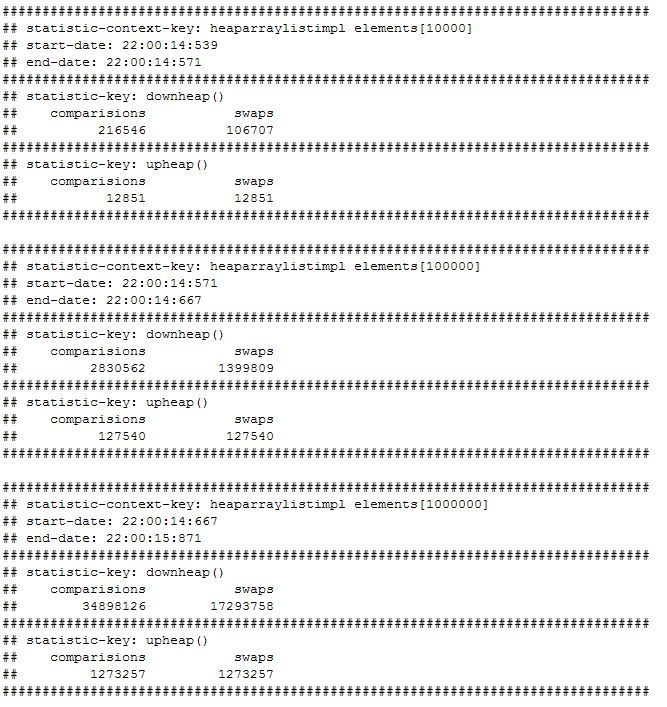
\includegraphics[scale=0.8]{\imagesDir/tests_heap_console_5.JPG}
  \caption
   {Diese Abbildung zeigt die Statistiken für das aufsteigende Sortieren von 10.000, 100.000, 1.000.000 Elementen}
\end{figure}
\newpage
\begin{figure}[h]
  \centering
  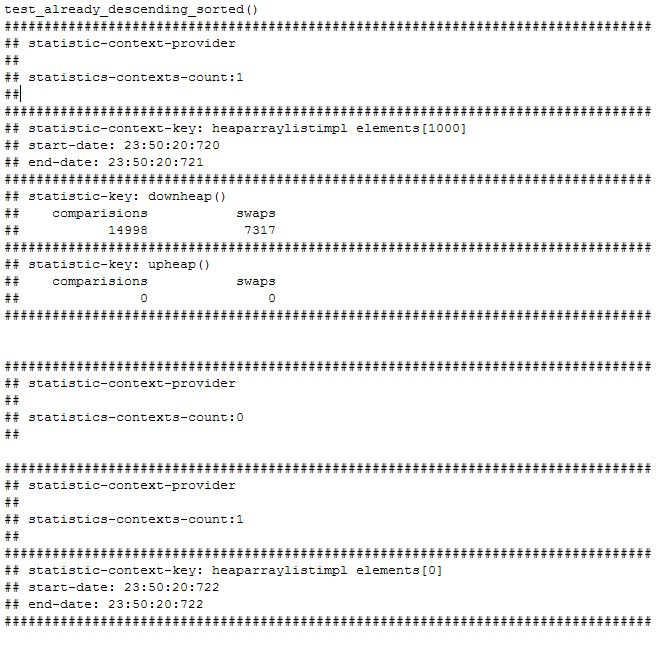
\includegraphics[scale=0.8]{\imagesDir/tests_heap_console_6.JPG}
  \caption
   {Diese Abbildung zeigt die Statistiken für das absteigende Sortieren 1.000 Elementen die bereits absteigend sortiert sind}
\end{figure}
\begin{figure}[h]
  \centering
  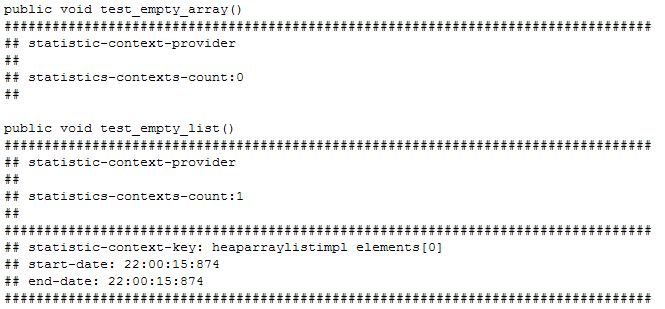
\includegraphics[scale=0.8]{\imagesDir/tests_heap_console_7.JPG}
  \caption
   {Diese Abbildung zeigt die Statistiken für das Sortieren einer leeren Liste und eines leeren Arrays}
\end{figure}
% =============================================
% 2.2 WucikSorter
% =============================================
% Idea (quicksorter)
% =============================================
\newpage
\subsection{QuickSorter}
Folgend ist die Lösungsidee für die QuickSorter Implementierung angeführt.\\
Diese Implementierung soll ebenfalls das Interface \inlinecode{Sorter<E>} implementieren und die CodeStatistics verwenden.\\
Entweder soll der Algorithmus so gewählt werden dass er aufsteigend und absteigend sortieren kann, oder die  Liste soll bei der inversen Sortierung mittels \inlinecode{Collections.reverse(list)} umgedreht werden.\\
Ansonsten ist der QuickSort Algorithmus wie bekannt zu implementieren.
% =============================================
% Source(quicksorter)
% =============================================
\newpage
\subsubsection{Source Code}
Folgend ist der Source der QuickSorter Implementierung angeführt.
\lstinputlisting[style=sourceFileStyle]{\mainPackage/sort/quick/QuickSorter.java}
% =============================================
% Tests (quicksorter)
% =============================================
\newpage
\subsubsection{\testSection}
Folgend sind die Test für die QuickSort Implementierung angeführt.
\testCommonText\\
\testSortCommonText
\begin{figure}[h]
  \centering
  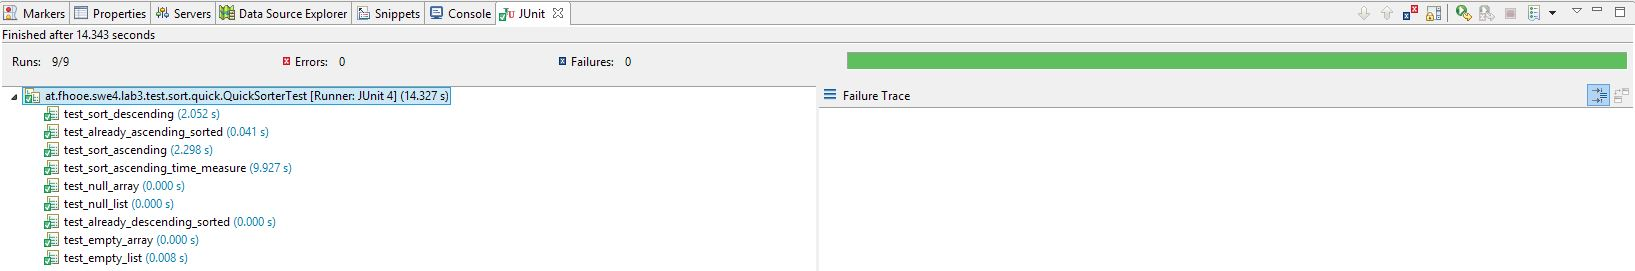
\includegraphics[width=\textwidth]{\imagesDir/tests_quick_junit.JPG}
  \caption
   {Diese Abbildung zeigt das Resultat der JUnit Tests im Eclipse}
\end{figure}
\newpage
\begin{figure}[h]
  \centering
  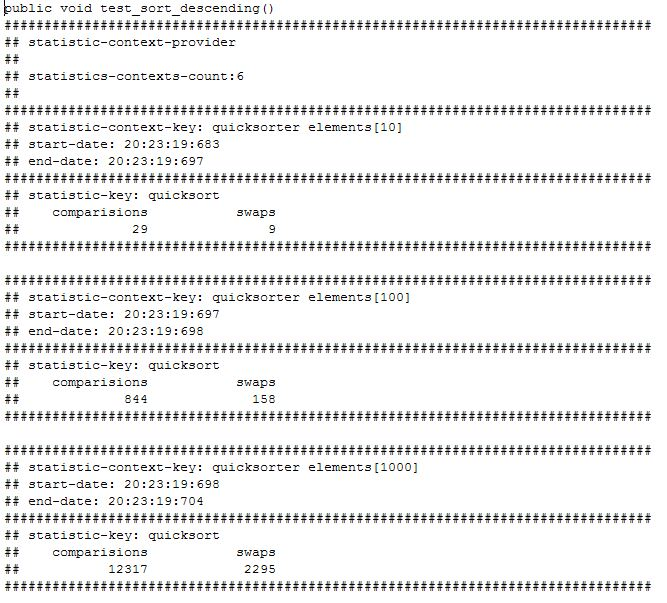
\includegraphics[scale=0.8]{\imagesDir/tests_quick_console_1.JPG}
  \caption
   {Diese Abbildung zeigt die Statistiken für das absteigende Sortieren von 10, 100, 1.000 Elementen}
\end{figure}
\newpage
\begin{figure}[h]
  \centering
  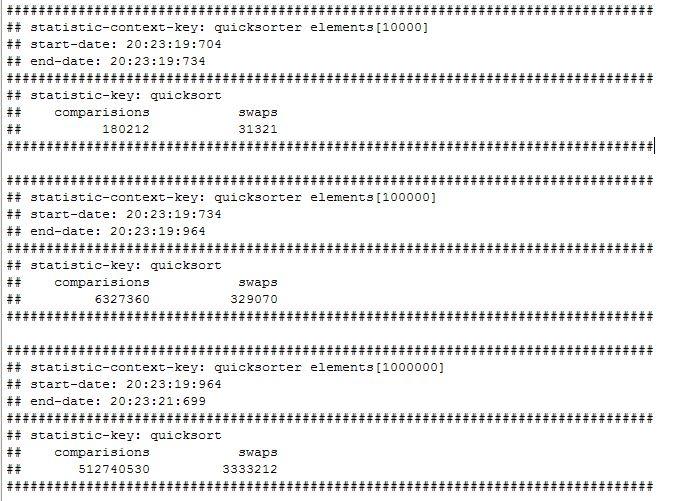
\includegraphics[scale=0.8]{\imagesDir/tests_quick_console_2.JPG}
  \caption
     {Diese Abbildung zeigt die Statistiken für das absteigende Sortieren von 10.000, 100.000, 1.000.000 Elementen}
\end{figure}
\newpage
\begin{figure}[h]
  \centering
  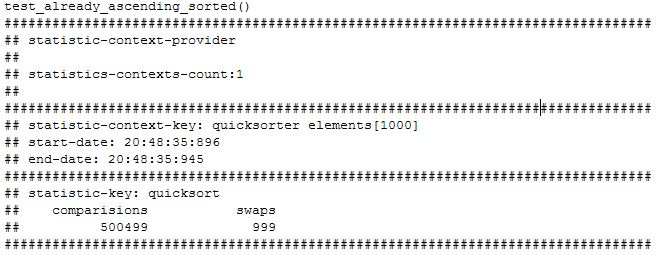
\includegraphics[scale=0.8]{\imagesDir/tests_quick_console_3.JPG}
  \caption
{Diese Abbildung zeigt die Statistiken für das aufsteigende Sortieren von 1.000 Elementen, die bereits aufsteigend sortiert sind}
\end{figure}
\newpage
\begin{figure}[h]
  \centering
  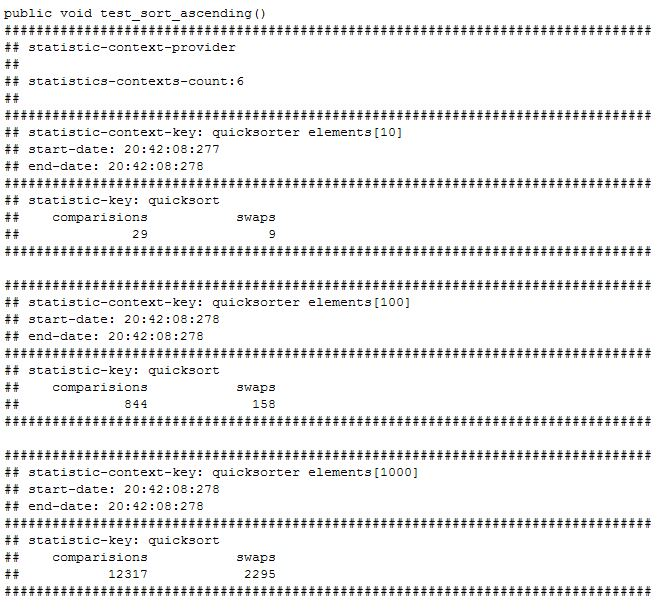
\includegraphics[scale=0.8]{\imagesDir/tests_quick_console_4.JPG}
  \caption
   {Diese Abbildung zeigt die Statistiken für das aufsteigende Sortieren von 10, 100, 1.000 Elementen}
\end{figure}
\newpage
\begin{figure}[h]
  \centering
  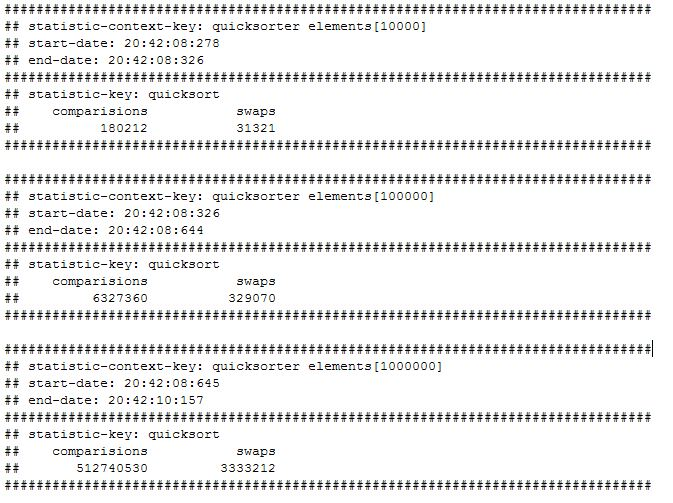
\includegraphics[scale=0.8]{\imagesDir/tests_quick_console_5.JPG}
  \caption
  {Diese Abbildung zeigt die Statistiken für das aufsteigende Sortieren von 10.000, 100.000, 1.000.000 Elementen}
\end{figure}
\newpage
\begin{figure}[h]
  \centering
  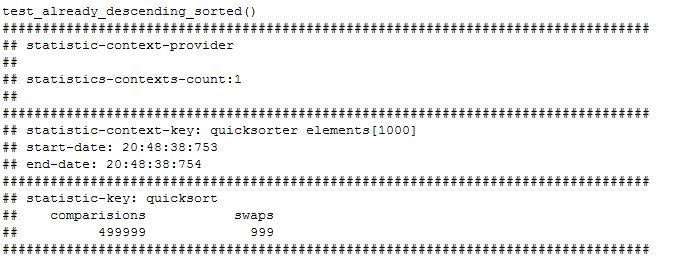
\includegraphics[scale=0.8]{\imagesDir/tests_quick_console_6.JPG}
  \caption
   {Diese Abbildung zeigt die Statistiken für das absteigende Sortieren von 1.000 Elementen, die bereits absteigend sortiert sind}
\end{figure}
\newpage
\begin{figure}[h]
  \centering
  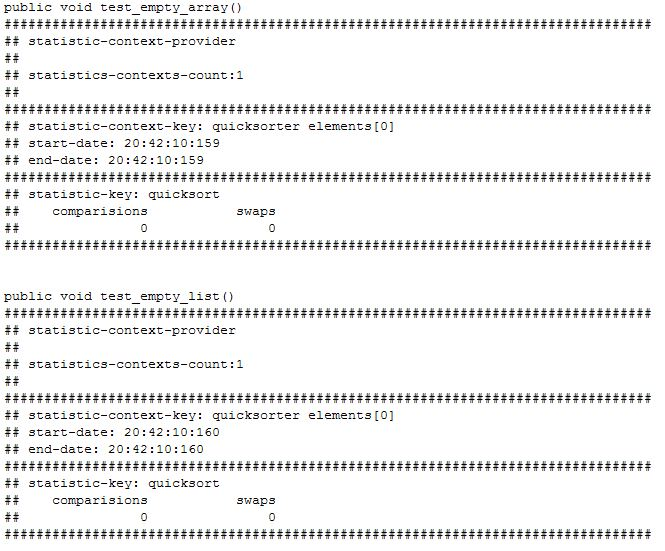
\includegraphics[scale=0.8]{\imagesDir/tests_quick_console_7.JPG}
  \caption
   {Diese Abbildung zeigt die Statistiken für das Sortieren von einer leeren Liste und eines leeren Array}
\end{figure}

% =============================================
% 2.2 Zeitausertung
% =============================================
\newpage
{\color{myred}
	\section
		{Zeitauswertung}
}
Folgend sind die Zeitmessungen für den HeapSorter angeführt, wobei diese mit 1.000.000 Zufallswerten im Bereich von 1 - 100.000 mit einem seed \inlinecode|System.currentMillis()| generiert wurden.\\
{\color{myred}
ACHTUNG: Diese Test sind sehr zeitintensiv und beanspruchen die Maschine stark. Abhängig von der Hardware könnten Probleme auftreten bzw. diese Tests sehr lange dauern.
}
\begin{figure}[h]
  \centering
  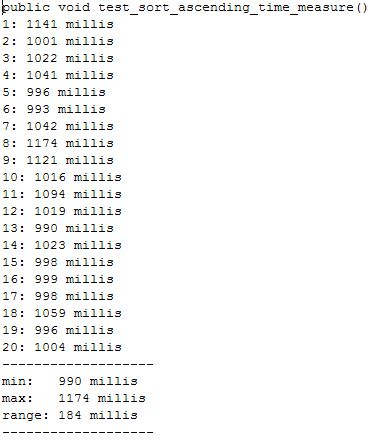
\includegraphics[scale=0.7]{\imagesDir/tests_heap_console_8.JPG}
  \caption
   {Diese Abbildung zeigt die Zeitmessungen des HeapSorter Algorithmus}
\end{figure}
\begin{figure}[h]
  \centering
  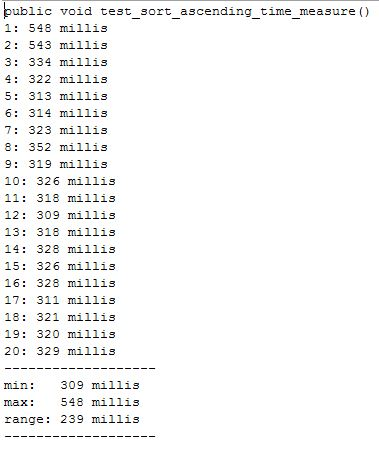
\includegraphics[scale=0.7]{\imagesDir/tests_quick_console_8.JPG}
  \caption
   {Diese Abbildung zeigt die Zeitmessungen des QuickSorter Algorithmus}
\end{figure}
\\
Es ist zu sehen das der QuickSorter Algorithmus um den Faktor 3 schneller ist als der Heapsorter Algorithmus, daher ist dieser vorzuziehen. Bei mehreren Durchläufen hat sich auch gezeigt, dass die Zeiten der Sortierung der ersten Male beim QuickSorter länger dauern als die anderen Durchläufe, was ich auf die Laufzeitumgebung zurückführe.
\end{document}  